При детальном изучении временной задержки нельзя пренебречь линзированием на отдельных звёздах в галактике. Этот эффект называется микролинзированием. Его масштабы (то есть характерные углы отклонения света) в миллион раз меньше масштабов обычного линзирования. На текущий момент разрешить микро-изображения (множественные изображения, возникающие в результате микролинзирования) на таких расстояниях не представляется возможным. Однако вполне возможно “засечь” микролинзирование благодаря кратковременному увеличению яркости отдельных объектов. 

\section{Программа \tt{microlens}}
    В данной работе для изучения микролинзирования используется вычислительная программа {\tt{microlens}} (\cite{wambsganss1999}), которая моделирует методом обратной трассировки лучей (\textit{inverse ray tracing}) распределение каустик в плоскости источника, основываясь на распределении звёзд в плоскости линзы. Выходными данными этой программы являются карты микрокаустик, содержащие значения обусловленного микролинзированием усиления. Основными параметрами для каждой карты являются поверхностные плотности звёзд $\sigma_*$\footnote{В этой главе поверхностная плотность, определяемая выражением \eqref{convergence}, обозначается символом $\sigma.$} и непрерывно распределенной тёмной материи $\sigma_c$ в линизирующей галактике, внешний сдвиг $\gamma$, учитывающий вклад гравитационного потенциала скопления галактик, а также функция масс звёзд. 

\begin{figure}[H]
    \centering
	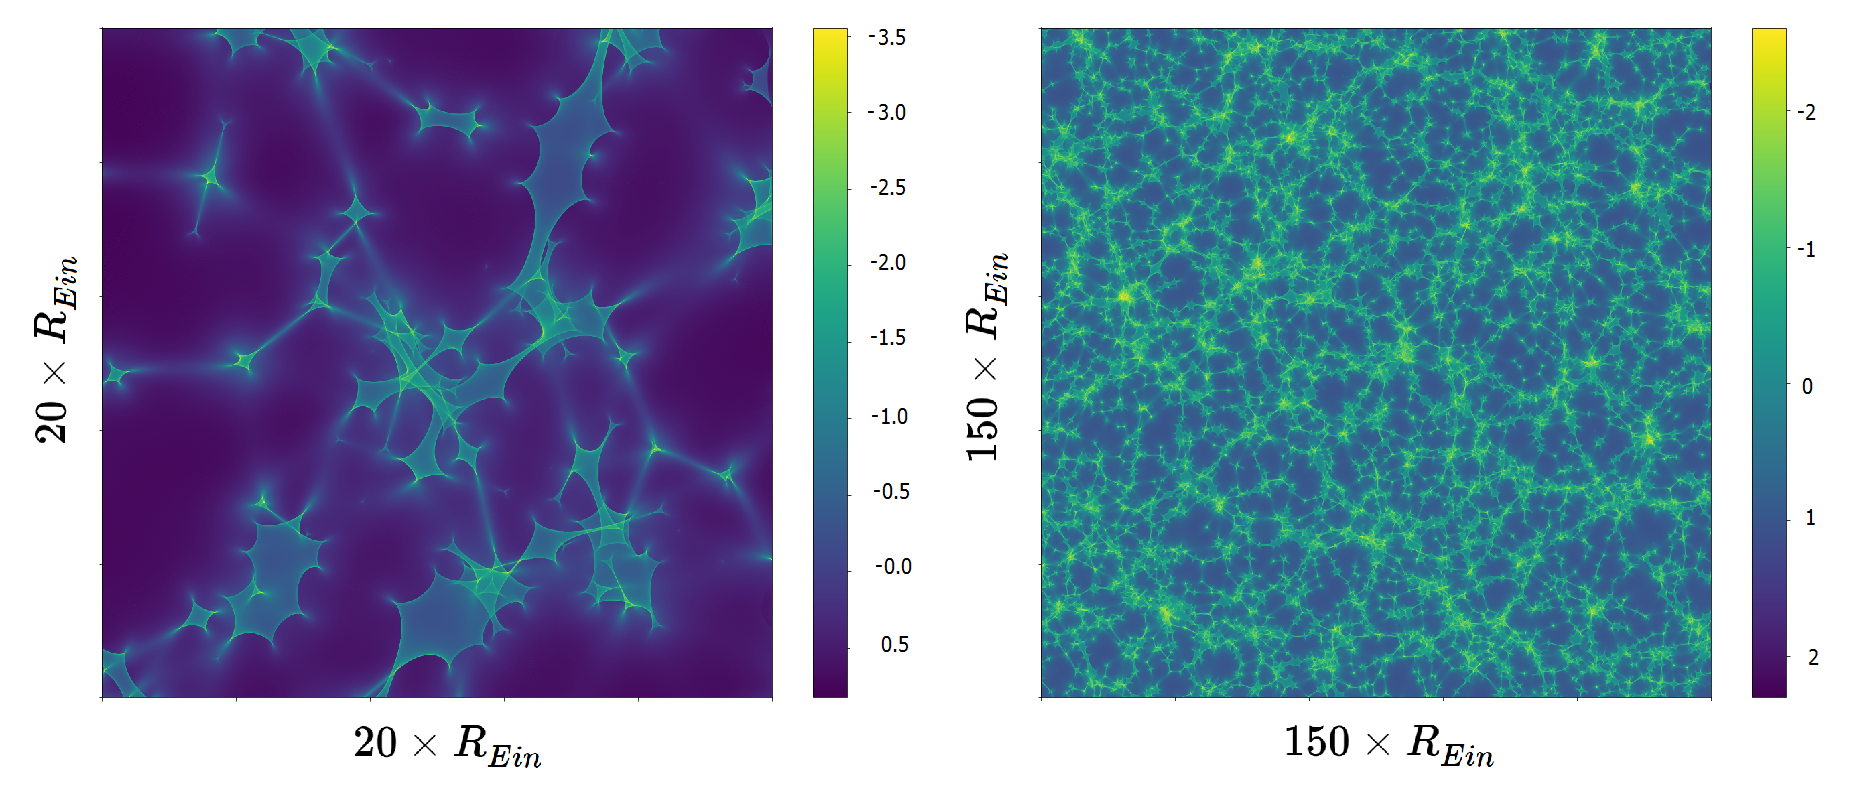
\includegraphics[scale=0.22]{pics/maps_example.png}
	\caption{Карты микрокаустик. Количество звёзд-линз слева - 313, справа - 14526. Цветовая шкала (в единицах звёздных величин) показывает, как увеличивается или ослабляется яркость источника вследствие микролинзирования только. \label{fig:micromaps}} 
\end{figure}
Здесь и далее для простоты предполагается, что все звезды в галактике имеют одинаковую массу, которая равна массе Солнца. На Рисунке \ref{fig:micromaps} приведены примеры результатов выполнения программы {\tt{microlens}} - карты усилений для двух различных значений количества звёзд, вызывающих микролинзирование. Светлые области означают, что источник усиливается, находясь в них, тёмные - что ослабляется. Видно, что а) сеть каустик намного богаче при большем количестве звёзд-линз, б) по всей карте усиление меняется и почти нигде не остаётся таким, каким его предсказывает модель линзы, то есть в отсутствие микролинзирования.
    
\section{Влияние микролинзирования на усиление изображений точечного источника}
    Чтобы наглядно показать вклад микролинзирования в изменение звёздной величины \textbf{точечного источника}, используется подход, аналогичный изложенному в работе \cite{shwamb2002}. Для изображённых на Рисунке \ref{fig:histograms} карт микролинзирования (слева) были построены гистограммы (справа), по сути, являющиеся плотностью вероятности микролинзирования и характеризующие усиление или ослабление видимой звёздной величины источника. Для всех трех проиллюстрированных случаев полная поверхностная плотность галактики-линзы остается постоянной, меняется лишь вклад звезд в полную массу системы.

\begin{figure}[H]
    \centering
	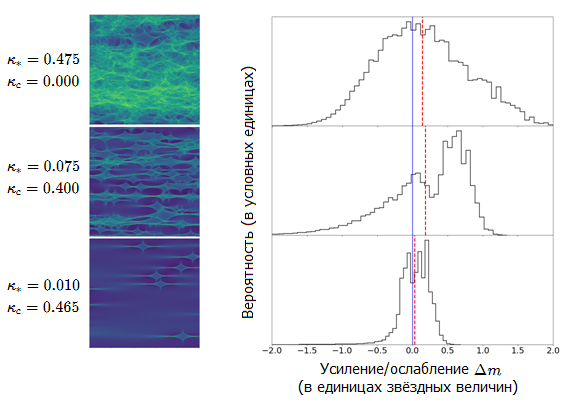
\includegraphics[scale=0.75]{pics/histograms.png}
	\caption{\texit{Слева}: карты микрокаустик, количество звёзд уменьшается сверху вниз. Размер каждой карты - $20 \times 20 R_{Ein}$. \textit{Справа}: соответствующие этим картам плотности вероятности микро-усилений (т.е. изменений звездной величины источника вследствие микролинзирования только). Сплошная голубая линия показывает $\Delta m=0$, т.е. когда звездная величина источника согласуется с теоретически ожидаемым значением макро-усиления (вследствие линзирования галактикой как целым), пунктирная красная линия - среднее по карте значение усиления. \label{fig:histograms}} 
\end{figure}

Так как микролинзирование происходит на отдельных звёздах, при уменьшении их количества (при этом величина $\sigma_*+\sigma_с$, то есть полная поверхностная плотность, сохраняется постоянной) дисперсия плотности вероятности ожидаемо уменьшается. Ещё один вывод, который отсюда можно сделать: микролинзирование в среднем ослабляет изображение (по крайней мере, для того набора параметров, который используется для построенных карт). 

    
\section{Влияние размера источника на микролинзирование}
    Как известно, микролинзирование при больших размерах источника вносит несущественный вклад в блеск источника (\cite{schneider1992}). Для того, чтобы оценить размер источника, начиная с которого вкладом микролинзирования можно пренебречь, мы оценили величину стандартного отклонения микро-усилений в звездных величинах mobs как функцию размера источника. 

Для этой цели было сгенерировано 10 различных карт микрокаустик, каждая со следующими параметрами: $\sigma_*=0.4, \sigma_c = 0$, размер - $ 150 \times 150 $ радиусов Эйнштейна, разрешение - 1000x1000 пикселей. Источник моделировался кругом с постоянной поверхностной яркостью. Для различных значений радиусов источника производилась операция свёртки (\textit{convolution}) с каждой из построенных карт, в результате чего на выходе получалась новая карта с учётом неточечности источника. Далее, для каждого значения радиуса источника вычислялось стандартное отклонение  $\delta m_{o b s}$ по следующей формуле: 
\begin{equation}
\delta m_{o b s}=\sqrt{\frac{1}{N} \sum_{i=1}^{N}\left(x_{i}-\overline{x}\right)^{2}},
\end{equation}
где N - количество элементов в выборке, полученной объединением всех карт, $x_i$ - значения усилений, $\overline x$- среднее значение усиления по выборке.

Полученная зависимость приведена на Рисунке 4. Пунктирной линией показана теоретическая оценка стандартного отклонения микро-усилений для больших источников (угловой размер которых превышает 5 радиусов Эйнштейна) из работы (\cite{refsdalstabell1991}l):

\begin{equation}
\delta m_{o b s} \approx \frac{2.17 \sqrt{|\sigma|}}{\theta s}
\end{equation}
где $\sigma$ - плотность звёзд, $\theta_s$ - размер источника в единицах радиуса Эйнштейна для характерной массы звезды. Формула предполагается справедливой при $\gamma=0, \sigma < 1$. 

\begin{figure}[H]
    \centering
	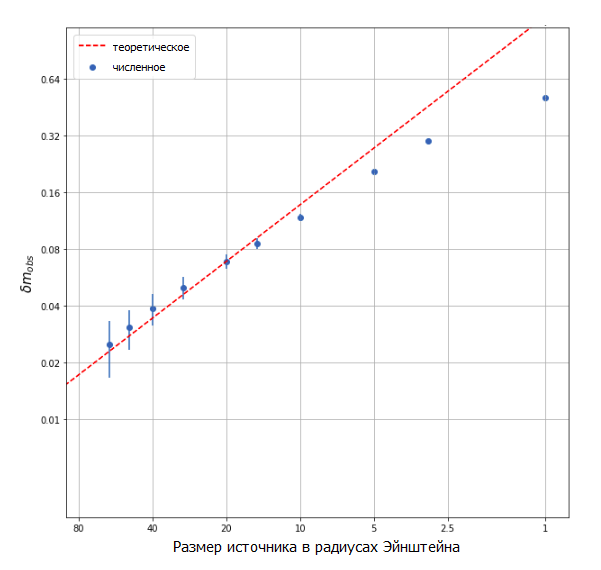
\includegraphics[scale=0.75]{pics/size_np_std.png}
	\caption{ Рис.5 Зависимость стандартного отклонения mobsот среднего значения усиления. Пунктирной линией показана теоретическая оценка $\delta m (\theta_s)$ для источников с $\theta_s > 5$(\cite{refsdalstabell1991}). Плотность звёзд: $\sigma_*=0.4$. Плотность тёмной материи и внешний сдвиг: $\sigma_с=0$.  } 
\end{figure}
Видно, что при увеличении размера источника на порядок, m уменьшается примерно так же на порядок, из чего можно сделать вывод, что для больших источников микролинзирование несущественно.
    
\section{SN Refsdal и микролинзирование}
    Как обсуждалось выше, микролинзирование может вносить существенный вклад в наблюдаемую кривую блеска, если размер источника не превышает радиус Эйнштейна $theta_E$ для звезды-микролинзы. Для конфигурации SN Refsdal (см. Рис. \ref{fig:snrefsdalfig}) оценим $\theta_E$ для звезды с массой $1 M_{\odot}$. Расстояния до галактики-линзы (члена скопления MACSJ1149.6+2223, $z_L=0.54$), до источника ($z_S=1.49$), а также между линзой и источником равны, согласно формуле \eqref{ang_dia_dist}, 
$$ D_d=D_A(0,z_L)=1311.54 \ \textrm{МПк}, $$
$$ D_s=D_A(0,z_S)=1744.81 \ \textrm{МПк}, $$
$$ D_{ds}=D_A(z_L,z_S)=932.47 \ \textrm{МПк}, $$
соответственно. В результате, радиус Эйнштейна для звезды с массой $1 M_{\odot}$ составляет, согласно формуле \eqref{r_ein}, $\theta_E = 2 \cdot 10^{-6}$ угловых секунд.

Для сверхновых II типа максимальный размер фотосферы составляет $R_{SN} \sim 10^{15}$ см (\cite{razmer}), или, в угловых единицах, $\theta_{SN} \sim 3 \cdot 10^{-7}$ угловых секунд. Таким образом, угловой размер SN Refsdal не превышает характерный радиус Эйнштейна, 
а значит, микролинзирование может вносить существенные искажения в её кривые блеска.